\section{Numerical way to perform convolution}
\subsection{Discrete convolution}

Usually when dealing with real life signals, we don't have the complete function in but rather, discreet samples of the function. So it is also useful to look at the discrete convolution, which is given by,

\begin{align*}
    y[k] = (f*h)[k] = \sum_{m=0}^{\infty} f[m]h[m-k]
\end{align*}

Discrete colvolution follow all properties continuous convolution follows. we use this to numeically compute convolution of two signals.

\subsection{Convolution Theorem}

The convolution theorem states that,

If,
\begin{align*}
    (u*v)(t) = r(t)
\end{align*}

Then,
\begin{align*}
    \mathcal{L}\{r(t)\} = \mathcal{L}\{u(t)\}\mathcal{L}\{v(t)\}
\end{align*}

This provides a much faster way to compute convolution of the signals.

\subsection{Fast Fourier Transform (FFT) and it's inverse (IFFT)}

FFT is the algorithm used to find the fourier transform of a given signal. It is a recursive algorithm with a time complexity of $\mathcal{O}(n\log(n))$. To explain the algorithm and explain how convolution theorem works, we can explain it using product of two polynomials.

Let $P_1(x)$ and $P_2(x)$ be polynomials of degree $n$. Let $\vec{p_1}$ and $\vec{p_2}$ be the vectors, whose elements are the coefficients of $P_1(x)$ and $P_2(x)$.
If $P(x) = P_1(x)\times P_2(x)$, then the coefficients of $P(x)$ is the discrete convolution of $\vec{p_1}$ and $\vec{p_2}$. We can verify that with some algebra.

It is also known that, through $n$ unique points, there is a unique polynomial of degree $n$ passing through it. Using this property, let us choose $2n$ points on each of $P_1$ and $P_2$, with the x-coordinates. That will give us, $P_{1_p} = [(x_0, P_1(x_0)), (x_1, P_1(x_1), \dots)]$ and $P_{2_p} = [(x_0, P_2(x_0)), (x_1, P_2(x_1), \dots)]$, which we will call the point form of the polynomials. Now if we multiply the results, we will end up with $2n$ unique points that lie on $P(x)$ (i.e., $P_p = [(x_0, P_1(x_0)\times P_2(x_0)), (x_1, P_1(x_1)\times P_2(x_1)), \dots]$). Now if we find the polynomial that is passing through these points, that will give us the polynomial we needed all along.
In a nutshell, the process of finding the unique points on each polynomial to be multiplied is FFT and finding the equation of the polynomial from it's point form is IFFT.

Now, to find the point form by chosing random values of x and computing for each of them is pretty inefficient. Thus, we will look at something symmetric, so that the computations can be reduced.

Let,
\begin{align*}
    P(x) = a_0x^n + a_1x^{n-1} + \dots + a_n\\
    P(x) = P_e(x^2) + xP_o(x^2)\\
    P(-x) = P_e(x^2) -xP_o(x^2)
\end{align*}
where, $P_e(x)$ is the polynomial made only with the even terms of the original polynomial, and $P_o(x)$ is the polynomial made only with the odd terms of the polynomial, with the common $x$ term taken out.
With this, finding $P(x)$ for n points become simpler, as it will be enough to calulate $P_e$ and $P_o$ n/2 points. It would be really convenient if we could do such splitting for $P_e$ and $P_o$, but $x^2$ breaks the symmetry, and requires it to be complex. Well, whatif, we make it complex? And this is how the FFT algorithm works.

In the simplest case, where $n=2^k,k\in \mathbb{N}$, we take the $n/2^{th}$ root of 1, and recursively find $P_e$ and $P_o$.

The peudocode of FFT looks like the following:

\begin{algorithm}[!ht]
\caption{Fast Fourier Transform (FFT)}
\begin{algorithmic}[1]
\Procedure{FFT}{$x$}
    \State $n \gets |x|$ \Comment{Length of the input array}
    \If{$n = 1$} 
        \State \Return $x$
    \EndIf
    
    \State $\omega \gets e^{-2\pi i / n}$ \Comment{Note: negative exponent in Python code}
    \State $P_e \gets (x_0, x_2, \ldots, x_{n-2})$ \Comment{Even-indexed elements}
    \State $P_o \gets (x_1, x_3, \ldots, x_{n-1})$ \Comment{Odd-indexed elements}
    
    \State $y_e \gets \text{FFT}(P_e)$ \Comment{Recursive call on even-indexed elements}
    \State $y_o \gets \text{FFT}(P_o)$ \Comment{Recursive call on odd-indexed elements}
    
    \State $y \gets $ complex array of zeros of length $n$ \Comment{Initialize output array}
    \For{$i = 0$ to $n/2 - 1$}
        \State $y_i \gets y_e[i] + \omega^i \cdot y_o[i]$ \Comment{First half}
        \State $y_{i+n/2} \gets y_e[i] - \omega^i \cdot y_o[i]$ \Comment{Second half}
    \EndFor
    
    \State \Return $y$
\EndProcedure
\end{algorithmic}
\end{algorithm}

Now, that we finally know how to perform FFT, we can multiply the outputs to get the convolution. But there is a problem with the above algorithm. To calculate the convolution of 2 functions with n discrete samples, our convolved output will have 2n points. But the above algorithm gives n points, and thus multiplying the n points element wise, will only give us n points in the convolved signal. So, we need to modify it such that it gives us 2n points.


\begin{algorithm}[!ht]
\caption{Fast Fourier Transform (FFT) - For convolution}
\begin{algorithmic}[1]
\Procedure{FFT}{$x$}
    \State $n \gets |x|$ \Comment{Length of the input array}
    \If{$n = 1$} 
    \State \Return $(x, -x)$
    \EndIf
    
    \State $\omega \gets e^{-\pi i / n}$ \Comment{Note: observe it's $2n^{th}$ root of unity.}
    \State $P_e \gets (x_0, x_2, \ldots, x_{n-2})$ \Comment{Even-indexed elements}
    \State $P_o \gets (x_1, x_3, \ldots, x_{n-1})$ \Comment{Odd-indexed elements}
    
    \State $y_e \gets \text{FFT}(P_e)$ \Comment{Recursive call on even-indexed elements}
    \State $y_o \gets \text{FFT}(P_o)$ \Comment{Recursive call on odd-indexed elements}
    
    \State $y \gets $ complex array of zeros of length $n$ \Comment{Initialize output array}
    \For{$i = 0$ to $n - 1$}
        \State $y_i \gets y_e[i] + \omega^i \cdot y_o[i]$ \Comment{First half}
        \State $y_{i+n} \gets y_e[i] - \omega^i \cdot y_o[i]$ \Comment{Second half}
    \EndFor
    
    \State \Return $y$
\EndProcedure
\end{algorithmic}
\end{algorithm}


Now that we have the fourier transform of our signals, and multiplied them, we have the transformed version of the convolved signal. Now we have to apply the inverse Fourier Transform over it. How are we to do it?

Fourier Transform of a discreet signal can be considered as a matrix multiplication.


\begin{align*}
\begin{bmatrix}
    X(\omega^0)\\
    X(\omega^1)\\
    \vdots\\
    X(\omega^n)
\end{bmatrix} 
    &=
\begin{bmatrix}
    1      & 1      & \dots  & 1\\
    1      & \omega & \dots  & \omega^{n-1}\\
    \vdots & \vdots & \vdots & \vdots\\
    1      & \omega^{n-1} & \dots & \omega^{(n-1)(n-1)}
\end{bmatrix}
\begin{bmatrix}
    x_0\\
    x_1\\
    \vdots\\
    x_{n-1}
\end{bmatrix}\\
\begin{bmatrix}
    x_0\\
    x_1\\
    \vdots\\
    x_{n-1}
\end{bmatrix}
    &=
\begin{bmatrix}
    1      & 1      & \dots  & 1\\
    1      & \omega & \dots  & \omega^{n-1}\\
    \vdots & \vdots & \vdots & \vdots\\
    1      & \omega^{n-1} & \dots & \omega^{(n-1)(n-1)}
\end{bmatrix}^{-1}
\begin{bmatrix}
    X(\omega^0)\\
    X(\omega^1)\\
    \vdots\\
    X(\omega^n)
\end{bmatrix}\\
\begin{bmatrix}
    x_0\\
    x_1\\
    \vdots\\
    x_{n-1}
\end{bmatrix}
    &=
    \frac{1}{n}
\begin{bmatrix}
    1      & 1      & \dots  & 1\\
    1      & \omega^{-1} & \dots  & \omega^{-(n-1)}\\
    \vdots & \vdots & \vdots & \vdots\\
    1      & \omega^{-(n-1)} & \dots & \omega^{-(n-1)(n-1)}
\end{bmatrix}
\begin{bmatrix}
    X(\omega^0)\\
    X(\omega^1)\\
    \vdots\\
    X(\omega^n)
\end{bmatrix}\\
\end{align*}

Notice how the matrix looks very identical except that the roots of unity are inverted, and the whole matrix is divided by n. So with minor modifications to the FFT algorithm, we can perform IFFT too.

\begin{algorithm}
\caption{Inverse Fast Fourier Transform}
\begin{algorithmic}[1]
\Procedure{IFFT-Recursive}{$x$}
    \State $n \gets |x|$ \Comment{Length of the input array}
    \If{$n = 1$} 
        \State \Return $x$
    \EndIf
    
    \State $\omega \gets e^{2\pi i / n}$ \Comment{Note: opposite sign that of FFT for IFFT}
    \State $P_e \gets (x_0, x_2, \ldots, x_{n-2})$ \Comment{Even-indexed elements}
    \State $P_o \gets (x_1, x_3, \ldots, x_{n-1})$ \Comment{Odd-indexed elements}
    
    \State $y_e \gets \text{IFFT-Recursive}(P_e)$ \Comment{Recursive call on even-indexed elements}
    \State $y_o \gets \text{IFFT-Recursive}(P_o)$ \Comment{Recursive call on odd-indexed elements}
    
    \State $y \gets $ complex array of zeros of length $n$ \Comment{Initialize output array}
    \For{$i = 0$ to $n/2 - 1$}
        \State $y_i \gets y_e[i] + \omega^i \cdot y_o[i]$ \Comment{First half}
        \State $y_{i+n/2} \gets y_e[i] - \omega^i \cdot y_o[i]$ \Comment{Second half}
    \EndFor
    
    \State \Return $y$
\EndProcedure

\Procedure{IFFT}{$X$}
    \State $y \gets \text{IFFT-Recursive}(X)$
    \State \Return $y / |X|$ \Comment{Scale by $1/n$}
\EndProcedure
\end{algorithmic}
\end{algorithm}

\begin{figure}[H]
    \centering
    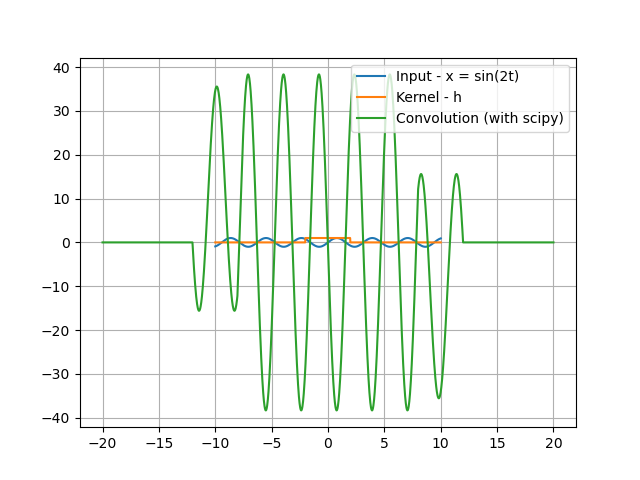
\includegraphics[width=0.7\linewidth]{figs/sci.png}
    \caption{Convolution by scipy}
\end{figure}

\begin{figure}[H]
    \centering
    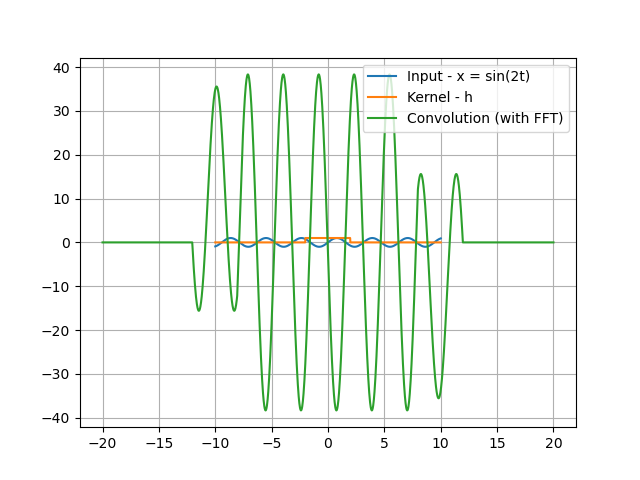
\includegraphics[width=0.7\linewidth]{figs/FFT.png}
    \caption{Convolution with python-implementation of FFT}
\end{figure}

\begin{figure}[H]
    \centering
    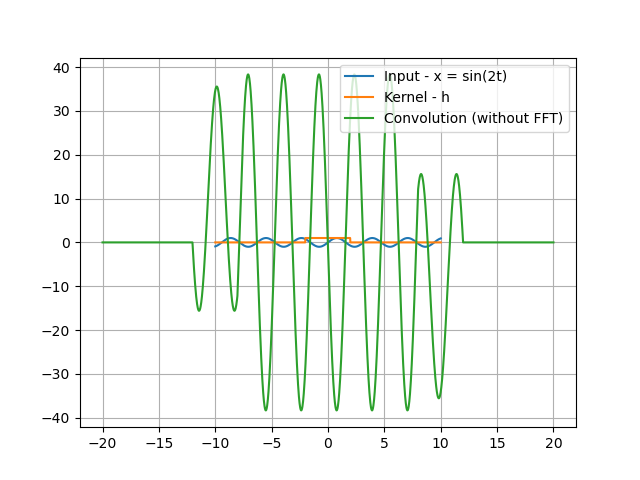
\includegraphics[width=0.7\linewidth]{figs/base.png}
    \caption{Convolution without FFT and IFFT algorithm}
\end{figure}

As we can see, the convolution matches. 


Now comparing the runtime of each algorithm,
\texttt{
Discreet Convolution:  0.33714938163757324\\
Scipy's Discreet Convolution 0.0010726451873779297\\
Discreen Convolution (FFT):  0.03110957145690918\\
}

Scipy's implementation is the fastest, as it is a professional tool with a lots of optimizations made. But as we can see, for the $n=1024$, FFT algorithm made convolution almost 10 times faster than regular convolution. Approximately, the time complexity of regular convolution is $\mathcal{O}(n^2)$ and FFT is $\mathcal{O}(n\log n)$, which  approximately matches.



	     
